%----------------------------------------------------------------------------
\chapter{Tervek és alternatívák}
\label{chapt:birdmap-introduction}
%----------------------------------------------------------------------------
Ebben a fejezetben bemutatom a fejlesztés előtti állapotot, amikor a munkám elején a fontosabb vizualizációs alternatívákat értékeltem.

%----------------------------------------------------------------------------
\section{Tervezés}
%----------------------------------------------------------------------------
A munkám elején egyeztettem a seregély riasztó keretrendszert fejlesztő kollégákkal, 
hogy ki tudjam választani a vizualizáció szempontjából legfontosabb komponenseket.
A jellemző adatvizualizációs megoldások közül az alábbi hármat találtam kulcsfontosságúnak a következő célokra:
\begin{itemize}
    \item \textbf{Hőtérkép}. Hasznos lenne egy olyan felület, ahol az eszközök GPS koordinátái és a seregély detektálást jelző üzenetek alapján, meg lehetne jeleníteni a seregélyek hozzávetőleges előfordulásának helyeit és gyakoriságát egy térképen, hőtérképes formában.
    \item \textbf{Eszköz állapotok}. Jelenleg a Command and Control mikroszolgáltatás felé indított kéréseken kívül, nincs lehetőség a kihelyezett eszközök állapotának vizsgálatára. Szükség lenne egy olyan felületre, ahol ezek állapotai láthatóak, esetleg dinamikusan is frissülnek.
    \item \textbf{Diagrammok}. A hőtérképen kívül egyéb olyan diagrammok is hasznosak lehetnek, ahol látható például, hogy melyik eszköz melyik percben észlelt madárhangot vagy, hogy egy eszköz összesen hány madárhangot észelt. Minnél több információ, annál jobb.
\end{itemize}
Ezeken kívül fontos követelmény volt még, hogy az alkalmazásom futtatható legyen Linux környezetben is, hogy az telepíthető legyen a Birbnetes Kubernetes \cite{kubernetes} klaszterébe.

Az alkalmazásom kapott egy nevet is, mely a Birbnetes-t és az említett hőtérképes ötletet ötvözve Birdmap lett.
\footnotetext{Microsoft Teams: Csevegő és gyülekezés tartó alkalmazás.}
%----------------------------------------------------------------------------
\section{Alternatívák}
%----------------------------------------------------------------------------
Az imént vázolt igények kielégítésére sok, széles körben alkalmazott megoldás létezik már, melyek jó példát mutattak a saját alkalmazásom fejlesztése során.

%----------------------------------------------------------------------------
\subsection{Grafana}
%----------------------------------------------------------------------------
A Grafana \cite{grafana} az egy nyílt forráskódú platformfüggetlen vizualizációs web alkalmazás.
Egy támogatott adatbázishoz csatlakoztatva különféle interaktív gráfokat és diagrammokat generál.
A testreszabhatóság maximalizásának érdekében különböző, akár harmadik fél által készített, bővítmények használatát is támogatja, 
melyekkel új adatforrások és panel típusok integrálhatók. 
A \ref{fig:grafana}-es ábra egy jó példa arra, hogy hogyan néz ki egy általános Grafana felület.

\begin{figure}[!ht]
    \centering
    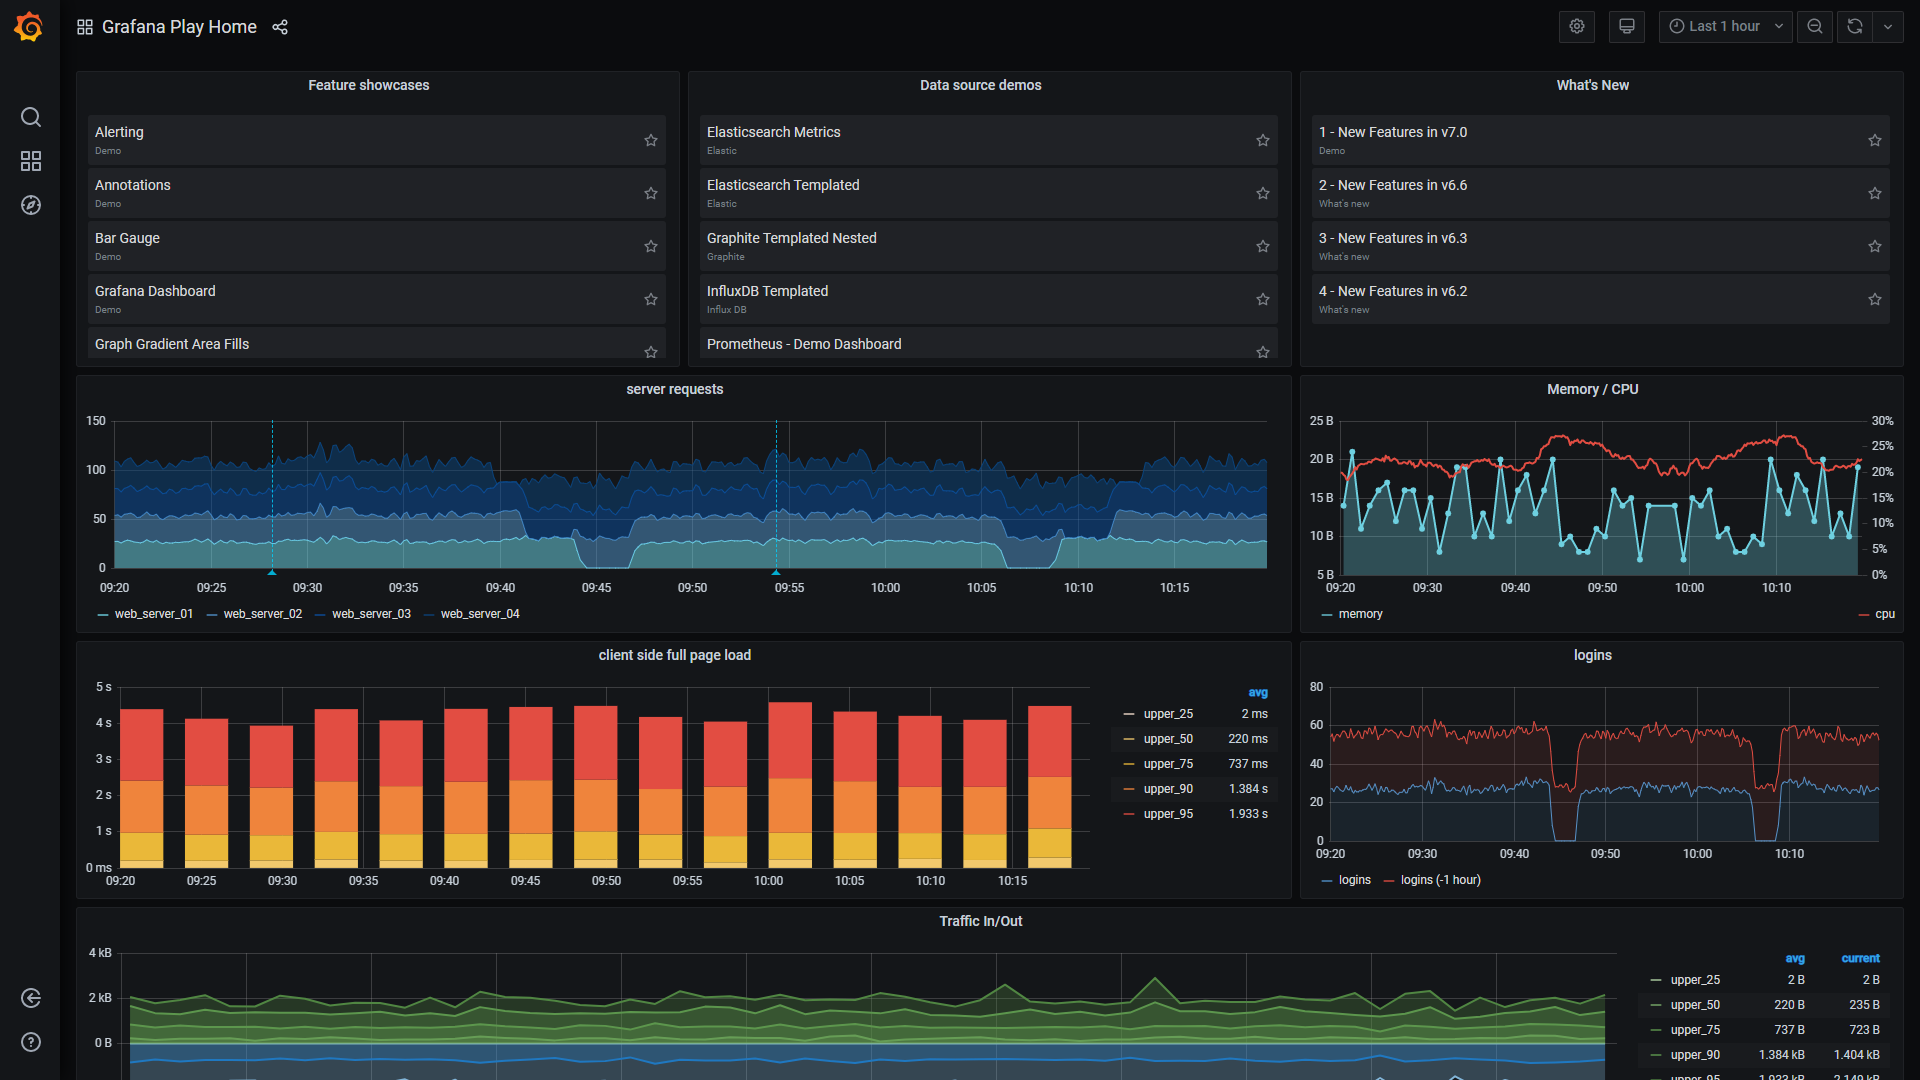
\includegraphics[width=150mm, keepaspectratio]{figures/grafana.png}
    \caption{A Grafana demo oldalának, a \url{https://play.grafana.org}-nak a felülete}
    \label{fig:grafana}
\end{figure}
    
%----------------------------------------------------------------------------
\subsection{Kibana}
%----------------------------------------------------------------------------
A Kibana \cite{kibana} jelentősen hasonlít a Grafanához, azonban amíg a utóbbit inkább az időben változó metrikák vizualizálására használják például processzor leterheltség vagy memória használat,
addig az előbbit elsődlegesen az Elasticsearch\footnote{Ingyenes és nyílt forráskódú index alapú keresőmotor} adatok, főként napló bejegyzések, analizálására használják.

\begin{figure}[!ht]
    \centering
    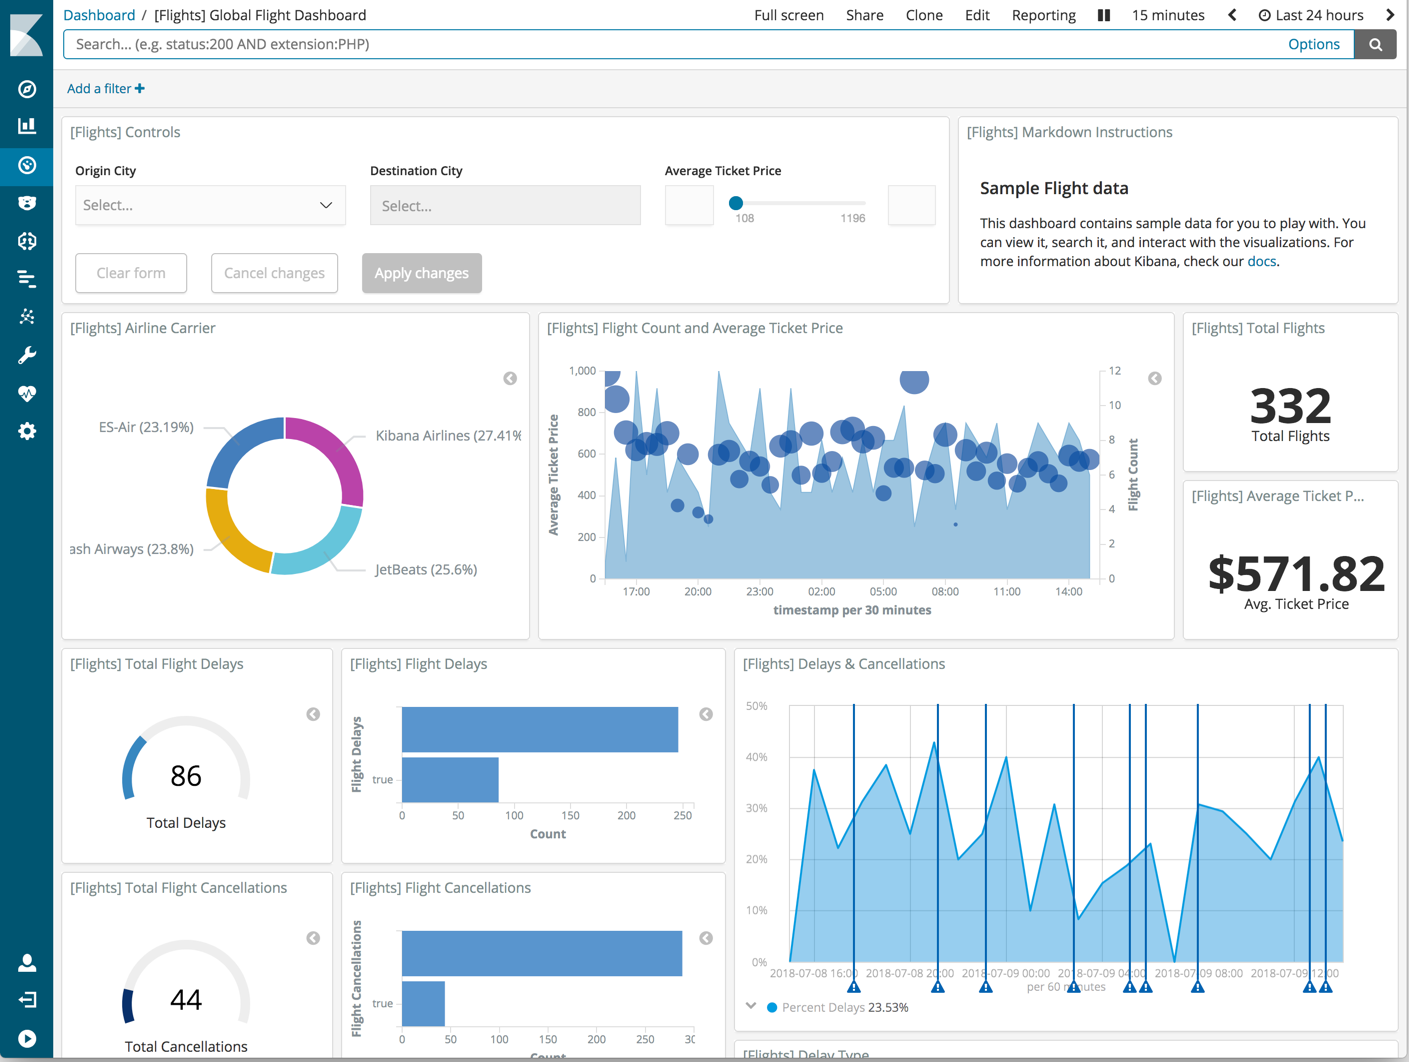
\includegraphics[width=150mm, keepaspectratio]{figures/kibana-dashboard.png}
    \caption{Egy példa a Kibana kezelőfelületére}
    \label{fig:kibana}
\end{figure}

%----------------------------------------------------------------------------
\subsection{Kubernetes Dashboard (Web UI)}
%----------------------------------------------------------------------------
A Kubernetes Dashboard \cite{kubernetes-dashboard} elsősorban nem a különböző adatok vizualizálását szolgálja, inkább a klaszter menedzselését próbálja egyszerűbbé és jobban áttekinthetővé tenni.
Azonban egy jó példa arra, hogy egy rendszer webes kezelőfelületének, milyennek is kell lennie.

\begin{figure}[!ht]
    \centering
    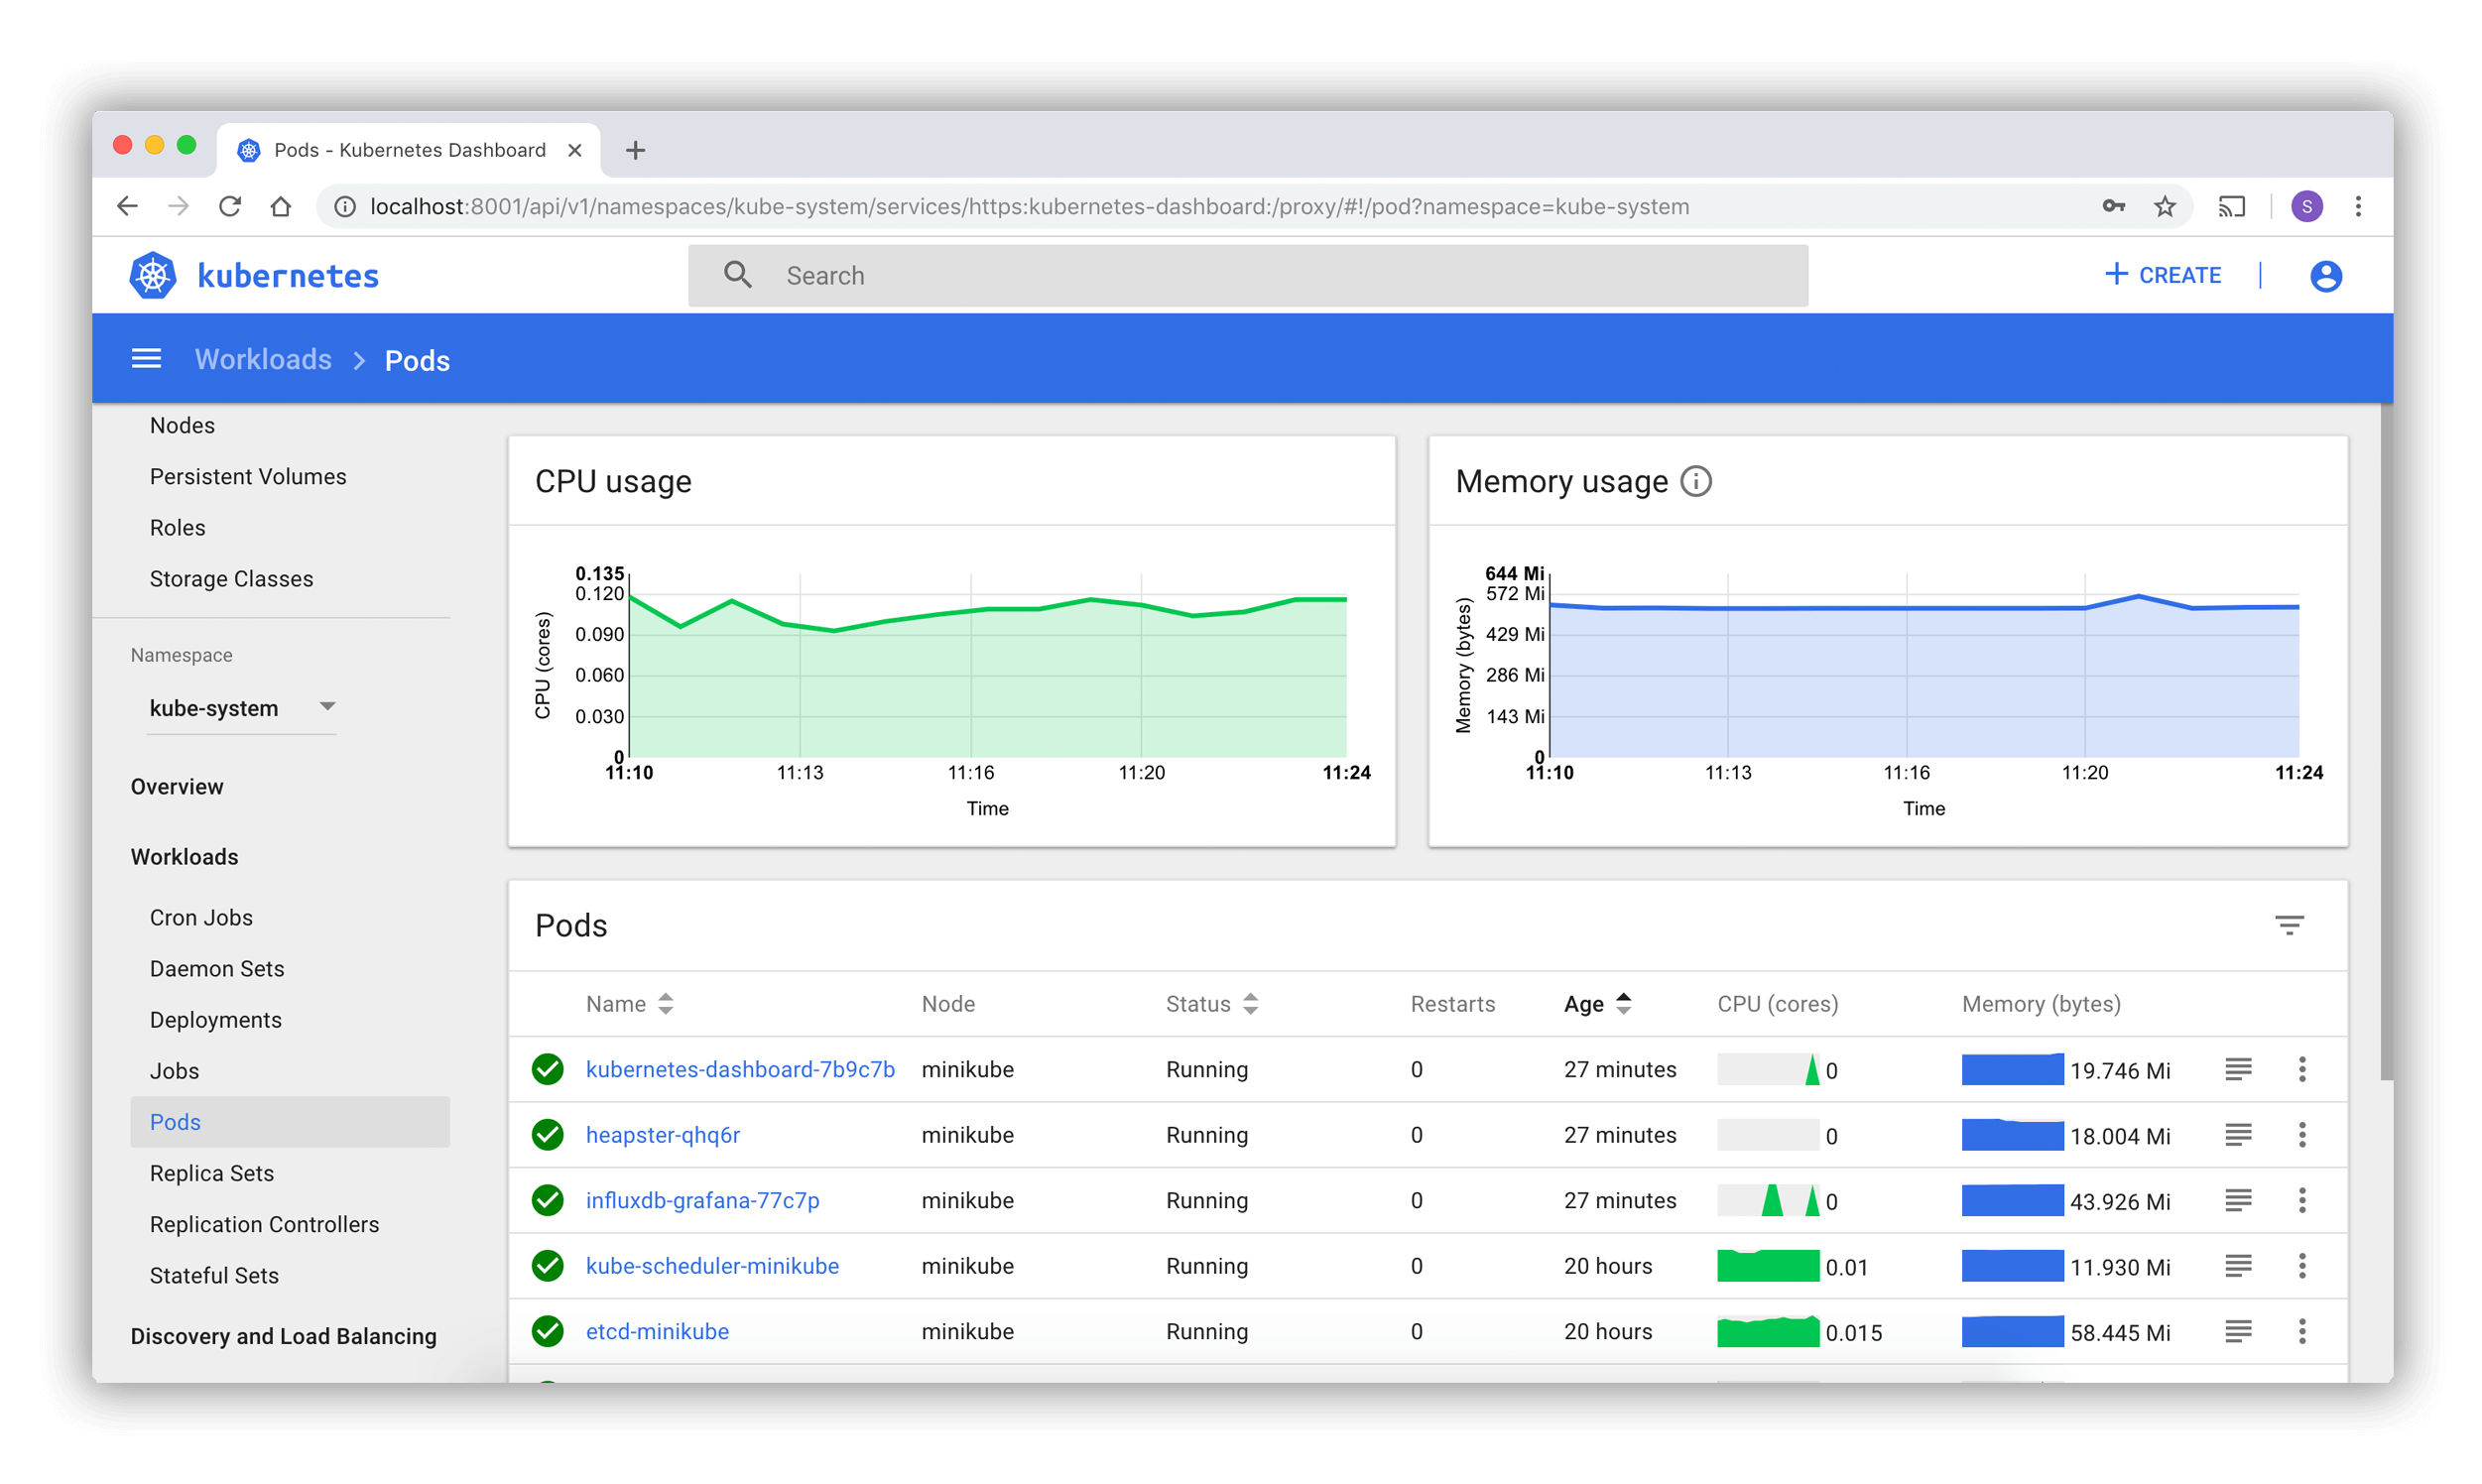
\includegraphics[width=150mm, keepaspectratio]{figures/kubernetes-dashboard.png}
    \caption{A Kubernetes Dashboard felülete}
    \label{fig:kibana}
\end{figure}